\newpage
\section{Messung grundlegender elektrischer Größen}\label{sec:01}

\subsection{Widerstandsmessung I: Einzelmessung}\label{sec:01-1}

\begin{highlightblock}[Widerstand mit nur einer Messung bestimmen]
Ohmscher Leistungswiderstand, $R=\SI{68}{\ohm}, P_{\max}=\SI{50}{\watt}$
\begin{enumerate}[label=\textbf{\alph*:}, ref=\alph*]
    \item Strom oder Spannungsrichtig messen?\label{itm:P1-1}
    \item Passende Spannung wählen.\label{itm:P1-2}
    \item Kontrollieren, ob der systematische Fehler vernachlässigbar ist.\label{itm:P1-3}
    \item Garantiefehlergrenzen abschätzen.\label{itm:P1-4}
    \item Messung durchführen.\label{itm:P1-5}
\end{enumerate}
\end{highlightblock}\medskip

\marginref{\ref{itm:P1-1}}
Da der Widerstand sehr klein ist, wird für dessen Ermittlung eine
spannungsrichtige U-I-Messung durchgeführt
\cite[S.~183]{SchrüferElmar2022EM:M}.

\marginref{\ref{itm:P1-2}}
Um eine passende Spannung zu wählen, werden erst die Messbereiche der Geräte
abgeschätzt. Relevante Daten der verwendeten Messgeräte (Tabelle
\ref{tab:geraeteliste}; Pos 1, 2) sind die $\SI{100}{\milli\volt}$ über den Amperemeter shunt
und der Innenwiderstand des Voltmeters über alle Messbereiche $R_{iV} =
\SI{10}{\mega\ohm}$.

\begin{wrapfigure}[7]{r}{5cm}
\vspace{-20pt}\raggedleft
\captionsetup{justification=raggedleft, singlelinecheck=false, margin=10pt}
\begin{circuitikz}[scale=0.85, transform shape]
    \draw (0,0) to[voltage source, v<=$U$] (0,3) 
        to[ameter, i=$I_A$] (3,3) coordinate (k1)
        to[vmeter, v=$U_V$, i>^=$I_V$, *-*] (3,0) coordinate (k2) -- (0,0);
    \draw (k1) -- ++(1,0) to[R, l=$R$, i>^=$I_R$] ++(0,-3) -- (k2);
\end{circuitikz}
\caption{Spannungsrichtige\\U-I-Messung}\label{fig:u-i-spannungsrichtig}
\end{wrapfigure}

Daraus ergeben sich folgende Abschätzungen für den Messbereich in abhängigkeit der gewählten Spannung:

\begin{itemize}
    \item $U_V \sim U - \SI{200}{\milli\volt}$
    \item $I_A \sim (U - \SI{200}{\milli\volt}) \left(\dfrac{1}{R} + \dfrac{1}{R_{iV}}\right)$
\end{itemize}

Sei die gewählte Spannung $U=\SI{5}{\volt}$, so ergibt sich:

\begin{itemize}
    \item $U_V \sim \SI{4.8}{\volt} \implies \text{MB:}~\SI{20}{\volt}$
    \item $I_A \sim \SI{71}{\milli\ampere} \implies \text{MB:}~\SI{200}{\milli\ampere}$
\end{itemize}

\marginref{\ref{itm:P1-3}}
Aus der Schaltung~\ref{fig:u-i-spannungsrichtig} ergibt sich folgende
Gleichung für den gemessenen Widerstand:

\begin{equation}
R = \frac{U_V}{I_R} = \frac{U_V}{I_A-I_V} = \frac{U_V}{I_A-U_V/R_{iV}}
\label{eq:r-spannungsrichtig}
\end{equation}

Der systematische Fehler in der Strommessung wird hierbei durch den
Innenwiderstand des Voltmeters verursacht. Da aber aus $R \ll R_{iV}$ folgt,
dass $I_A \approx I_R$, ist der Fehler sehr gering, kann aber trotzdem
korrigiert werden, sofern $R_{iV}$ bekannt ist.

\marginref{\ref{itm:P1-4}}
Die Garantiefehlergrenzen der Messgeräte (Tabelle~\ref{tab:geraeteliste}; Pos 1, 2) sind für die gewählten Messbereiche:
\begin{itemize}
    \item Voltmeter: $u_{U_V} = \pm(\SI{0.05}{\percent} + 3 \text{ Digits})
        = \pm(\SI{0.05}{\percent} \cdot \SI{20}{\volt} + 3 \cdot \SI{0.001}{\volt})
        = \pm \SI{0.013}{\volt}$
    \item Amperemeter: $u_{I_A} = \pm(\SI{0.3}{\percent} + 3 \text{ Digits})
        = \pm(\SI{0.3}{\percent} \cdot \SI{200}{\milli\ampere} + 3 \cdot \SI{0.01}{\milli\ampere})
        = \pm \SI{0.63}{\milli\ampere}$
\end{itemize}

\newpage
\begin{wrapfigure}[13]{r}{5cm}
    \vspace{-12pt}\centering
    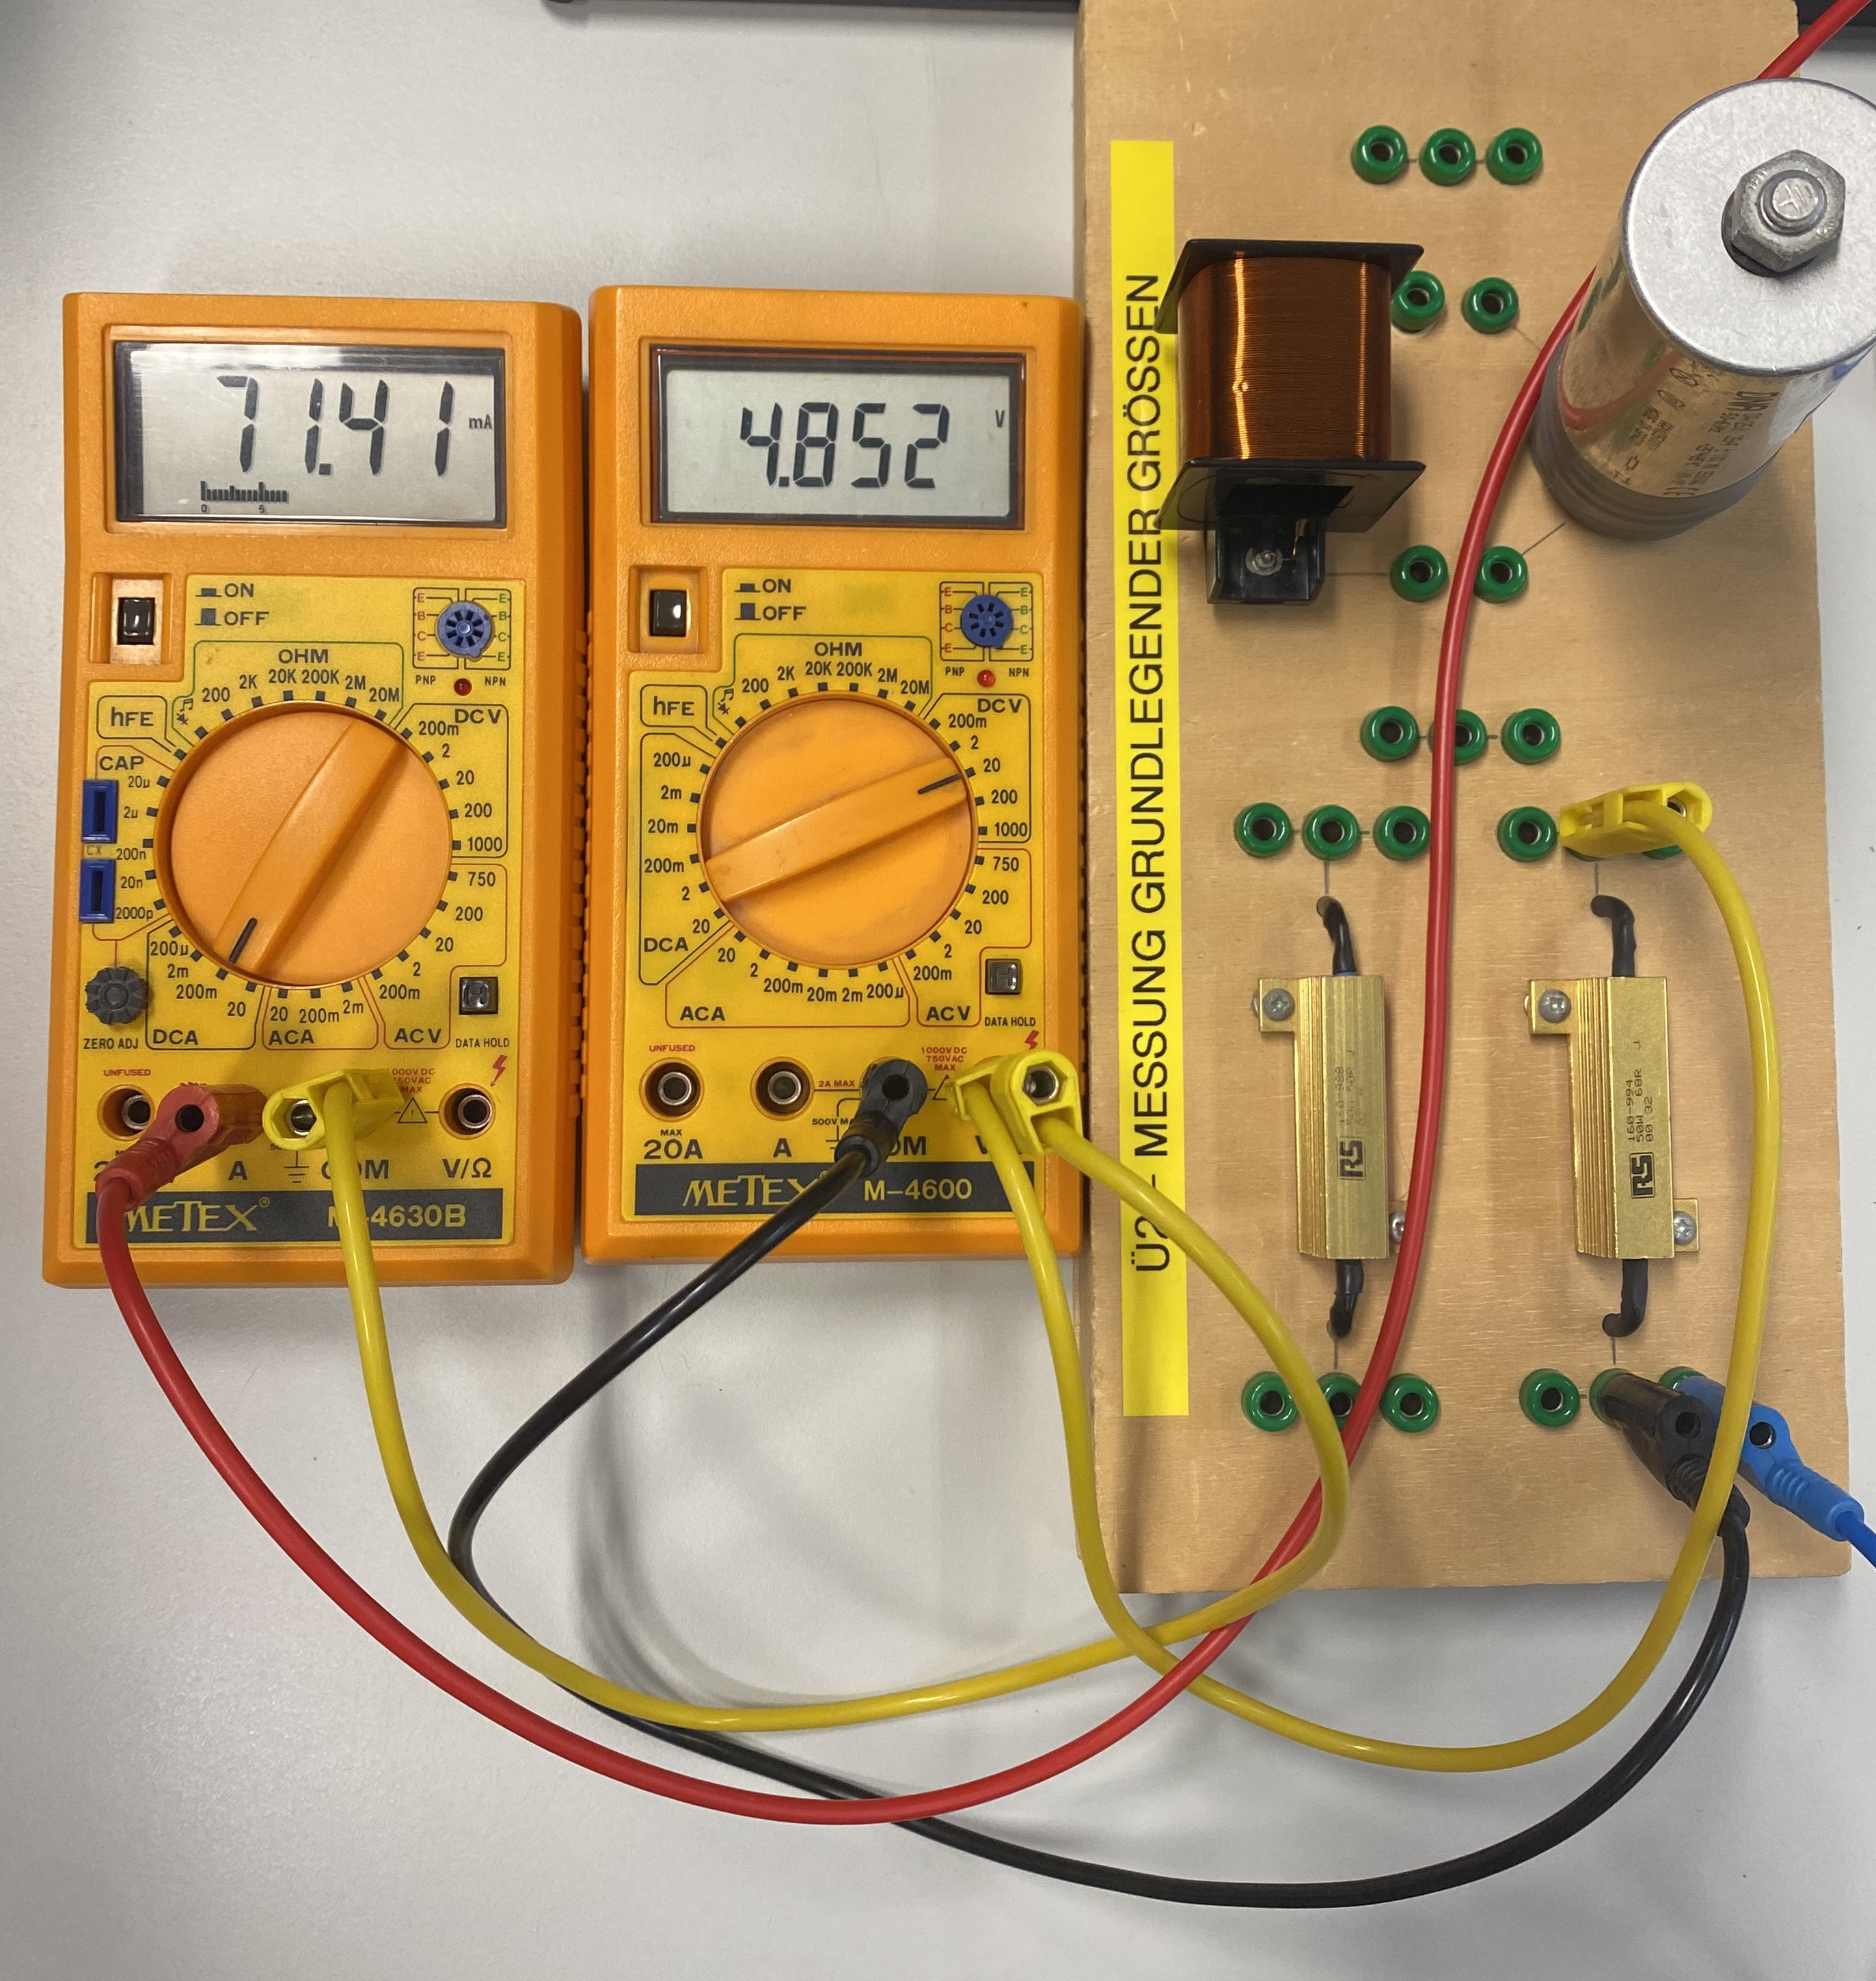
\includegraphics[width=5cm]{images/11_Aufbau.JPEG}
    \caption{Aufbau der Messung}\label{fig:11_aufbau}
\end{wrapfigure}

\marginref{\ref{itm:P1-5}}
Durchführung der Messung liefert die Messwerte für Strom und Spannung.
Anschließend wird der Widerstand mit Gleichung \ref{eq:r-spannungsrichtig} unter Anwendung der
Fehlerfortpflanzung~\cite[Gl.~1.80]{SchrüferElmar2022EM:M} berechnet.

\begin{itemize}
    \item $U_V = \SI{4.852}{\volt} \pm \SI{0.013}{\volt}$
    \item $I_A = \SI{71.41}{\milli\ampere} \pm \SI{0.63}{\milli\ampere}$ 
    \item $R = \SI{67.9}{\ohm} \pm \SI{0.6}{\ohm}$
\end{itemize}

Berechnung der Unsicherheit des Widerstandswertes:
\[
    u_R = \sqrt{{\left(\frac{\partial R}{\partial U}u_{U_V}\right)}^2 + {\left(\frac{\partial R}{\partial I}u_{I_A}\right)}^2} = \SI{0.6265}{\ohm}
\]
mit
\[
    \frac{\partial R}{\partial U}\Big|_{U=U_V} = \frac{I_A R_{iV}^2}{{(-I_A R_{iV} + U_V)}^2} =  \SI{14.00}{\ohm\per\volt}
\]
und
\[
    \frac{\partial R}{\partial I}\Big|_{I=I_A} = -\frac{U_{V}}{{(I_A - U_V/R_{iV})}^2} = -951.5 \si{\ohm\per\ampere}
\]